% $Author: ruben $
% $Date: 2010-05-09 22:31:50 $
% $Revision: 1.2 $

% For the FujabaDays 2006
\documentclass[submission,copyright,creativecommons]{eptcs}
\providecommand{\event}{TTC 2014} % Name of the event you are submitting to


\usepackage{graphicx,float,enumerate}
\usepackage{listings}
\usepackage{color}
\usepackage{wrapfig}

\graphicspath{{images/}}

\newcommand{\code}{\texttt}
\newcommand{\p}[1]{\textsf{#1}}


\setlength{\textwidth}{16.5cm}
\setlength{\oddsidemargin}{0cm}
\setlength{\evensidemargin}{0cm}
\setlength{\topmargin}{0cm}

\begin{document}

\definecolor{lightgray}{rgb}{.9,.9,.9}
\definecolor{darkgray}{rgb}{.4,.4,.4}
\definecolor{purple}{rgb}{0.5, 0, 0.33}
\definecolor{commentgreen}{rgb}{0.25,0.5,0.37} 
\definecolor{stringblue}{rgb}{0.16, 0, 1}
\definecolor{annotationgrey}{rgb}{0.39,0.39,0.39}


\lstdefinelanguage{Java}{
  keywords={typeof, try, long, void, new, true, false, catch, function, return,
  null, catch, switch, var, if, in, while, do, else, case, break, private, 
  protected,
  final, static, public, class, implements, extends, boolean, throws, throw,
  this, int, float, double}, 
  keywordstyle=\color{purple}\bfseries, ndkeywords={export}, 
  ndkeywordstyle=\color{darkgray}\bfseries,
  identifierstyle=\color{black},
  sensitive=true,
  comment=[l]{//},
  morecomment=[s]{/*}{*/},
  commentstyle=\color{commentgreen}\ttfamily,
  stringstyle=\color{stringblue}\ttfamily,
  morestring=[b]',
  morestring=[b]", 
  moredelim=[il][\textcolor{annotationgrey}]{$$},
  moredelim=[is][\textcolor{annotationgrey}]{\%\%}{\%\%}
}



\pagestyle{headings}

\title{The SDMLib solution to the Class Responsibility Assignment Case for TTC2016} 
\author{Christoph Eickhoff, Lennert Raesch, Albert Z{\"u}ndorf
\institute{
Kassel University, Software Engineering Research Group,\\
Wilhelmsh{\"o}her Allee 73, 34121 Kassel, Germany\\
\email{raesch|christoph|zuendorf@uni-kassel.de}
}}

\def\authorrunning{ Albert Z{\"u}ndorf}
\def\titlerunning{The SDMLib solution for TTC2016}

\maketitle

\begin{abstract}

This paper describes the SDMLib solution to the Class Responsibility Assignment Case 
for TTC2016. SDMLib provides reachability graph computation ala Groove. Thus, 
the simple idea was to provide rules for possible clustering operations and then use the
reachability graph computation to generate all possible clusterings. Then, we apply the
CRAIndex computation to each generated clustering and identify the best clustering. Of course,
this runs into scalability problems, very soon. Thus, we extended our reachability graph 
computation to do an A* based search space exploration. Therefore, we passed the CRAIndex 
computation as a metric to our reachability graph computation and in each step, we consider 
the set of not yet expanded graphs and choose the one, that has the best metric value for 
expansion. The paper reports about the results we achieved with this approach.  
   
  
\end{abstract}

\section{Introduction}
\label{sec:intro}

This paper describes the SDMLib solution to the Class Responsibility Assignment Case for TTC2016
\cite{ttc2016-case}. SDMLib provides reachability graph computation ala Groove 
\cite{rensink2003groove}. For a given start graph and a given set of rules, 
the reachability graph computation generates all graphs that may be derived from 
the start graph by applying all rules at all 
possibles matches as often as possible in all possible orders. Each time a new graph is 
computed, we search through the set of already computed graphs for an already known 
isomorphic graph. As proposed by \cite{rensink2003groove}, SDMLib computes node and graph 
certificates which are then used as hash keys to access potentially isomorphic graphs, 
efficiently. The node certificates then also help to do the actual isomorphism test. If a new 
graph has been generated, we create a so-called reachable state 
node and we connect the reachable state node of the predecessor graph with the reachable 
state node for the new graph via a rule application edge labeled with the name of 
the rule used. In addition, a root node of the graph is attached to the reachable state node. 
Altogether, the generated reachability graph has a top layer consisting of reachable 
state nodes connected via rule application edges and each reachable state node refers to 
the corresponding application graph via a \texttt{graphRoot} link. In SDMLib, this whole 
structure is again a graph, and graph rules may be applied to it in order to find e.g. 
reachable states with a maximal metric value for the attached application graph 
or to find states 
where all successor states have lower metric values or to find the shortest path leading to 
the best state. Actually, any graph related algorithm may be deployed.  

The Class Responsibility Assignment Case challenges the rule orchestration mechanisms 
provided by the different model transformation approaches. Thus, our solution uses the SDMLib 
reachability graph computation for rule orchestration. This is a very simple way to apply 
all rules in all possible ways and in addition we are able to investigate all intermediate 
results in order to identify which paths through the search space are the most interesting 
ones. The drawback of this approach is that it wastes a lot of runtime and memory space 
for copying the whole class model graph each time a rule is applied and for the search of 
already known isomorphic copies of the generated graphs. As shown in the case 
description, the number of possible clusterings grows with the Bell number, i.e. 
for larger examples a complete enumeration of all possible clustering is not possible in a 
meaningful time. As only a small fraction of the search space can be explored, it might be 
helpful to be able to investigate all intermediate states to identify the most promising spots 
for further expansion. Thus, we hope that the flexibility provided by the SDMLib reachability 
graphs to investigate different intermediate states pays off, at the end. 

As it is usually not possible to generate the whole reachability graph for a given example, 
our reachability graph computation may be restricted to a maximum number of reachable 
states to be considered. Next, we have extended our reachability graph computation with an A* 
like search space exploration that takes a metric as parameter and at each step chooses the 
state with the best metric value for expansion. We have developed two variants of this A* 
algorithm which will be discussed below. 

The next section introduces the rules we use to solve the Class Responsibility Assignment Case
and then Section~\ref{sec:expansion} shows the different search strategies we use in this 
example. Finally,~\ref{sec:results} shows our performance measurements. In the last section
we sum up our results. 
 
\section{The Model Transformation Rules}
\label{sec:rules}

Our feature clustering approach uses three SDMLib model transformation rules. In the 
preparation phase we use the rule shown in Figure~\ref{fig:RuleInitialClasses} to create 
one class for each feature in our class model. 

\begin{figure}[ht] \centering
	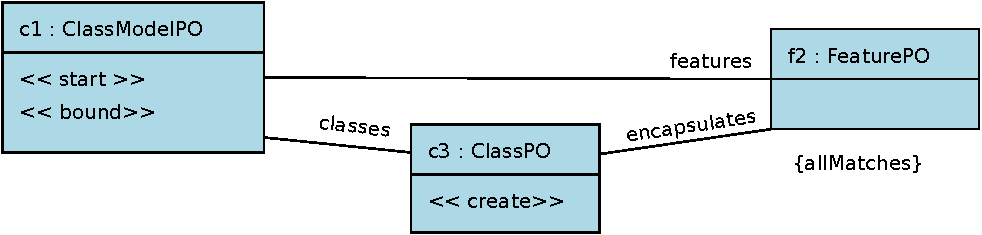
\includegraphics[width=\linewidth]{images/RuleAddInitialClasses.pdf}
 \caption{Rule adding initial classes}
 \label{fig:RuleInitialClasses}
\end{figure}

This rule starts by matching the pattern object \texttt{c1} to the 
\texttt{ClassModel} object passed as parameter. Then, \texttt{f2} is matched to a 
Feature object attached to this \texttt{ClassModel} object. The 
\texttt{\{allMatches\}} constraint causes the rule to be applied to all possible 
matches. Thus, for each \texttt{Feature} object in our current 
\texttt{ClassModel}, the \texttt {$<<$create$>>$ } sterotype on pattern object 
\texttt{c3} causes the creation of a new \texttt{Class} object. In addition 
the new \texttt{Class} object is attached to the \texttt{ClassModel} via a 
\texttt{classes} link and to the \texttt{Feature} object via an 
\texttt{encapsulates} link. Finally, the new \texttt{Class} object's \texttt{name} 
attribute gets assigned the concatenation of the prefix \texttt{"Class4"} 
and the \texttt{name} of the current \texttt{Feature}. Thus, after the 
execution of this rule, each feature has its own class containing just this 
feature. This class model is then used as starting point for the repetitive 
application of our clustering rules. 

We use two different clustering rules, one for clustering along attribute dependencies 
and one for clustering along method dependencies. Figure~\ref{fig:MergeAttributeRule} 
shows the attribute dependency clustering rule: 

\begin{figure}[ht] \centering
	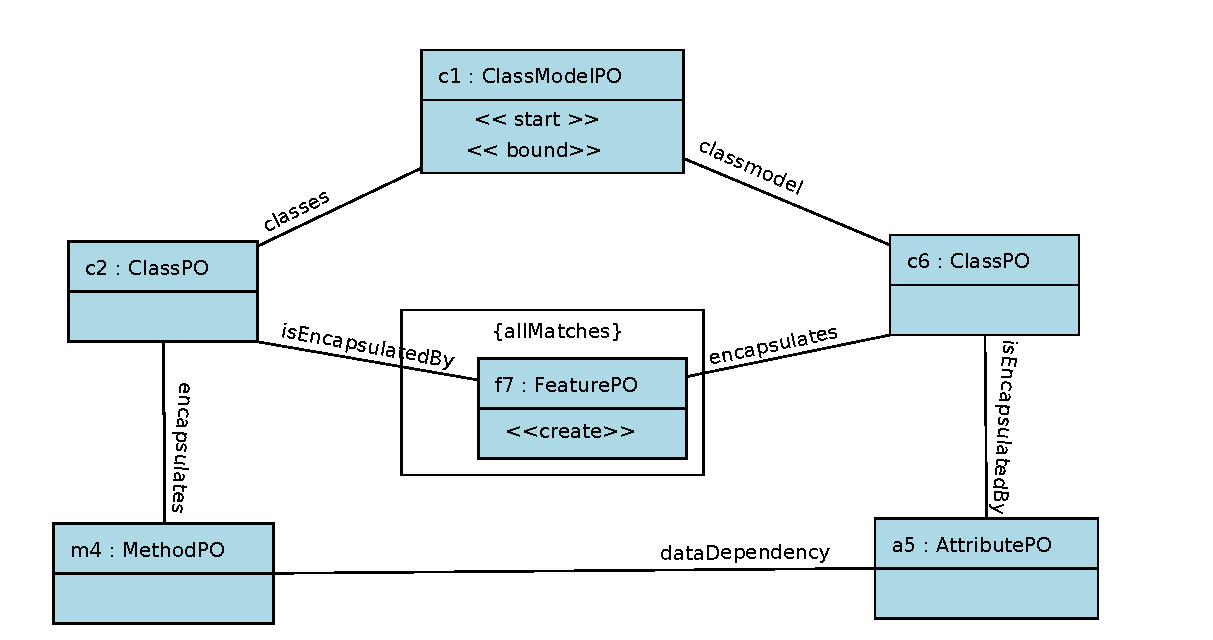
\includegraphics[width=\linewidth]{images/RuleMergeDataDep.pdf}
 \caption{Merging Classes via Attribute Dependencies}
 \label{fig:MergeAttributeRule}
\end{figure}  


\section{The Search Space Expansion Mechanisms}
\label{sec:expansion}

 


\begin{lstlisting}[language=Java, numbers=left, captionpos=b, 
label=Activity.initVariables.java, escapeinside={\%}{\%},
caption={General Reachability Graph Computation}
]
ReachabilityGraph::explore(depth) {
   todo = new ArrayList();
   todo.add(this.startState);
   states.put(certificate(this.startState), startState);
   while (! todo.isEmpty() && states.size() <= depth) {
      current = todo.get(0); todo.remove(0);
      for(Rule r : this.rules) {
         while (r.findMatch()) {
            newState = current.clone().apply(r);
            isoOldState = find(states, newState);
            if (isoOldState == null){
               states.put(certificate(newState), newState);
            	 addEdge(current, r, newState);
             	 todo.add(newState);
            } else {
               addEdge(current, r, isoOldState);
            }
         }
      }
   }
}

\end{lstlisting}


\section{Performance Results}
\label{sec:results}



\section{Summary}
\label{sec:summary}

 

\bibliographystyle{abbrv}
\bibliography{fujaba}  

\end{document}

 